%%=============================================================================
%% Methodologie
%%=============================================================================

\chapter{\IfLanguageName{dutch}{Methodologie}{Methodology}}
\label{ch:methodologie}

%% TODO: Hoe ben je te werk gegaan? Verdeel je onderzoek in grote fasen, en
%% licht in elke fase toe welke stappen je gevolgd hebt. Verantwoord waarom je
%% op deze manier te werk gegaan bent. Je moet kunnen aantonen dat je de best
%% mogelijke manier toegepast hebt om een antwoord te vinden op de
%% onderzoeksvraag.

In de vorige hoofdstukken werden de frameworks die in deze studie vergeleken
zullen worden geselecteerd en hun achtergrond besproken. In dit hoofdstuk wordt
de effectieve vergelijking tussen de verschillende frameworks gemaakt.
Verschillende belangrijke onderdelen van mobiele applicatieontwikkeling komen
aan bod tijdens de vergelijking. Voor elk framework wordt eerst de aanpak op dit
specifieke punt uitgelegd en vervolgens worden beide aanpakken met elkaar
vergeleken. In deze vergelijking worden enkel React Native en Flutter met elkaar
vergeleken, gezien er nog geen technische aspecten van .NET MAUI gekend zijn op
het moment van schrijven.


\section{Vergelijking eigenschappen}
\label{sec:vglEigenschappen}

Elk framework heeft zijn eigen eigenschappen en manier om bepaalde zaken aan te
pakken. In deze sectie worden de taal die gebruikt wordt binnen de frameworks en
de verschillende aanpakken op het gebied van navigatie, toegang tot de native
API's, opbouwen van de UI en de styling besproken.

\subsection{Taal framework}
\label{subsec:taalFramework}

Elk framework maakt gebruik van een bepaalde taal om een applicatie te
ontwikkelen. De taal van een framework is zeer belangrijk, aangezien het zowel
de sterke als minder sterke eigenschappen van een taal erft. Een framework met
een taal die traag is vergeleken met andere talen of die zeer ingewikkeld is om
te leren zal automatisch een minder goede keuze zijn. Het is dus zeer belangrijk
van beide talen te vergelijken.

\subsubsection{React Native}
\label{subsubsec:taalReactNative}

Zoals in sectie \ref{subsec:ReactNative} reeds besproken werd is React Native
gebaseerd op React, dat op zijn beurt gebaseerd is op JavaScript. JavaScript is
de meest gebruikte taal onder ontwikkelaars wereldwijd \autocite{Liu2020a}. Het
is een lichtgewicht taal die weinig eisen stelt aan de hardware van het systeem.
Het wordt vooral gebruikt voor de ontwikkeling van webpagina's, maar ook vele
andere omgevingen werken met JavaScript zoals o.a. Node.js. JavaScript bestaat
al sinds 1995 en is dus een zeer volwassen en stabiele programmeertaal.

Een zeer groot voordeel van JavaScript komt rechtstreeks voort uit het feit dat
het al lang bestaat en dat het zeer populair is: er zijn zeer veel libraries en
documentatie beschikbaar die het ontwikkelen van een applicatie sterk
vereenvoudigen.

Tot slot brengt de React basis nog een zeer groot voordeel met zich mee: de 'hot
reload'. React maakt gebruik van een virtual DOM, die een vereenvoudigde
beschrijving van de werkelijke DOM bijhoudt. Het aanpassen van de DOM is een
traag en intensief proces, het aanpassen van de virtual DOM is echter zeer snel
aangezien er niks getoond moet worden op het scherm hiervan. Bij het renderen
van een element wordt een snapshot genomen van de virtual DOM die de huidige
toestand van de virtual DOM bij houdt. Vervolgens wordt elk object in de virtual
DOM geüpdatet. Dit lijkt een intensieve operatie, maar door dat de virtual DOM
zo snel geüpdatet kan worden is het dit niet. Nu zijn er dus twee versies van de
virtual DOM, één van voor de update en één van erna. Beide versies worden met
elkaar vergeleken om vast te stellen wat er exact is veranderd. Enkel de
componenten die door de update aangepast zijn worden uiteindelijk in de echte
DOM ook aangepast. Door deze werkwijze moet er slechts een deel van de DOM
opnieuw gerenderd worden. Dit levert een grote tijdswinst op en stelt React in
staat om een 'hot reload' functie te hebben. Dit houdt in dat de UI direct
geüpdatet kan worden als de ontwikkelaar aanpassingen opslaat, zonder dat de
applicatie opnieuw gebuild moet worden. Er moet dus niet telkens op een nieuwe
build gewacht worden, wat bij native ontwikkeling wel het geval is en
minutenlang kan duren. Deze functionaliteit levert dus een grote tijdswinst op
tijdens het ontwikkelen!

\subsubsection{Flutter}
\label{subsubsec:taalFlutter}

De taal waarin Flutter applicaties geschreven worden, Dart, kwam al kort aan bod
in sectie \ref{subsec:Flutter}. Het is ontwikkeld door Google in 2011 maar is
pas in gebruik genomen buiten Google in 2017, toen Google Flutter uitbracht. Het
is een client-side programmeertaal die geoptimaliseerd is voor het maken van
UI's. Door dat het nog vrij recent is zijn er wel maar een beperkt aantal
libraries beschikbaar en moet de ontwikkelaar dus soms meer werk verrichten om
bepaalde zaken zelf te gaan schrijven. Verder is de documentatie soms ook
onvolledig en is er door de beperkte groep gebruikers slechts weinig
ondersteuning van de community.

Er zijn natuurlijk ook zeker enkele positieve eigenschappen aan Dart. Zo lijkt
de syntax zeer hard op Java en kan een ontwikkelaar die hier ervaring mee heeft
dus ook zeer snel aan de slag met Dart. 

Een ander voordeel is dat Dart zowel naar JavaScript als naar native machine
code gecompileerd kan worden. Naar JavaScript is handig voor het ontwikkelen van
een webapplicatie, omdat JavaScript een brede ondersteuning heeft in de meeste
browsers die Dart niet heeft. Voor het ontwikkelen van mobiele applicaties met
Flutter is het echter zeer handig dat het gecompileerd kan worden naar machine
code. Op deze manier worden prestaties van de applicatie bereikt die gelijk zijn
aan die van een native applicatie, ondanks de cross-platform ontwikkeling er
van!

Een laatste sterke eigenschap van Flutter is de 'hot reload' functie. Deze laat
toe om aanpassingen in de code (zoals updates in de UI, bug fixes of zelfs hele
nieuwe features) toe te passen op de applicatie zonder deze te moeten stoppen en
opnieuw builden. Voor zowel het ontwikkelen van de UI als het oplossen van
problemen is dit een zeer krachtige eigenschap die de ontwikkelingstijd dratisch
verlaagd. De werkwijze steunt op het bestaan van de Dart Virtual Machine. Dit is
een VM waar de Dart code in draait en die er voor zorgt dat de code wordt
omgezet naar de gewenste taal (machine code of JavaScript). De bron code
bestanden die geüpdatet zijn worden in deze VM geïnjecteerd en vervangen de
oudere versie van deze bestanden. Vervolgens wordt de hele widget tree opnieuw
opgebouwd, waardoor de aanpassingen getoond worden zonder dat de applicatie
gestopt moest worden.

\subsubsection{Vergelijking talen frameworks}
\label{subsubse:vglTalen}

Zoals in de vorige secties duidelijk werd steunen de twee frameworks op een
andere taal. In deze sectie worden de verschillen en gelijkinissen tussen beide
talen besproken.

Eerst en vooral moet er op gemerkt worden dat beide talen dezelfde achtergrond
hebben. Ze zijn beide gestart als een taal voor webomgevingen en zijn daarna
verder geëvolueerd om er meerdere soorten applicaties mee te kunnen schrijven.
Zo worden ze nu beide gebruikt voor de ontwikkeling van cross-platform
applicaties. Een groot verschil tussen de twee is echter dat JavaScript reeds
lang bestaat en dat Dart slechts zeer recent publiek gemaakt werd. Hierdoor is
er meer ondersteuning voor JavaScript dan voor Dart en zijn er voor JavaScript
veel meer libraries beschikbaar.

Een ander groot verschil is de syntax van de talen. JavaScript heeft een syntax
die voor beginnende programmeurs soms moeilijk kan zijn. De syntax van Dart
leunt zeer dicht aan bij deze van Java, die een stuk eenvoudiger is om te leren.
Beginnende programmeurs kunnen dus sneller aan de slag met Flutter dan met React
Native. Volgens \textcite{Liu2020a} is JavaScript echter de meest populaire
programmeertaal ter wereld, met 67,7\% van de ondervraagden die aangaven
JavaScript te gebruiken. Dart werd echter maar door 4\% van de ondervraagden
gebruikt! Vele ontwikkelaars hebben dus reeds een kennis van JavaScript en
kunnen sneller aan de slag met React Native dan met Flutter.

Flutter heeft een voordeel ten opzichte van React als het aankomt op de
prestaties  van de applicatie doordat de code gecompileerd kan worden naar
native machine code. JavaScript kan niet omgezet worden naar native machine
code, waardoor React Native gebruik moet maken van een brug tussen JavaScript en
de native machine code om te werken op een specifiek platform. Dit levert extra
overhead op, wat er voor zorgt dat de prestaties verminderen. 

Een gelijkenis tussen de twee frameworks is de hot reload functionaliteit. Ze
stellen beiden de ontwikkelaar in staat om aanpassingen zeer snel te kunnen
weergeven zonder dat de applicatie heropgestart hoeft te worden. Er bestaat wel
een verschil in aanpak tussen de twee. Bij React Native wordt er gebruikt
gemaakt van een virtual DOM om de staat van de UI voor en na de de update bij te
houden, zodat enkel de aangepaste componenten opnieuw hoeven gerenderd te
worden. Bij Flutter wordt er gebruikt gemaakt van een VM, die de aanpassingen
injecteert in de broncode en deze doorgeeft aan de applicatie, waarna de widget
tree opnieuw opgebouwd wordt. Hoewel beide frameworks de hot reload op een
andere manier aanpakken is het effect voor de ontwikkelaar hetzelfde:
aanpassingen kunnen meteen visueel gecontroleerd worden.


\subsection{Navigatie binnen de applicatie}
\label{subsec:navigatieApplicatie}

Een belangrijk deel van elke applicatie is de mogelijkheid om te kunnen
navigeren tussen verschillende pagina's van de applicatie. Elk cross-platform
framework moet dus de mogelijkheid voorzien om de ontwikkelaar toe te staan deze
functionaliteit te verwerken in de applicatie.

\subsubsection{React Native}
\label{subsubsec:navigatieReactNative}

React Native maakt voor de navigatie tussen de verschillende pagina's gebruik
van een library genaamd React Native Navigation. Dit is een standalone library
die de ontwikkelaar in staat stelt om zowel op Android als iOS navigatie aan te
leveren die een native uitstraling heeft. Het is één van de vele populaire
libraries binnen React Native die ontwikkeld zijn door de uitgebreide community
achter React Native. Onderliggend maakt deze library ook gebruik van een andere
library genaamd Animated om de animaties tijdens het navigeren naar een andere
pagina aan te bieden. De animaties en gebaren die gepaard gaan met het navigeren
kunnen volledig aangepast worden aan de voorkeuren van de ontwikkelaar. Er is
dus zeer veel vrijheid en de gebruiker krijgt een applicatie die navigeert zoals
een native applicatie. 

Om de navigatie te gebruiken moet de ontwikkelaar de hele applicatie wrappen in
een navigatiecontainer. Op deze manier heeft de library toegang tot de gehele
applicatie en kan de ontwikkelaar de navigatie tussen de verschillende pagina's
instellen naar wens. De werkwijze om de applicatie te wrappen met de
navigatiecontainer en de verschillende pagina's toe te voegen aan de
navigatiestack is te zien in figuur \ref{fig:opzettenNavigatieReactNative}.

\begin{figure}
    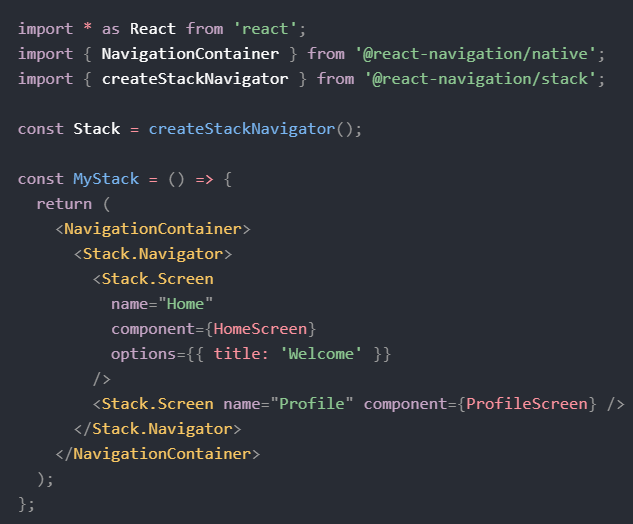
\includegraphics[width=\linewidth]{OpzettenNavigatieReactNative.png}
    \caption{Opzetten navigatie in een React Native applicatie. Bron:
        reactnative.dev/docs/navigation}
    \label{fig:opzettenNavigatieReactNative}
\end{figure}

Vervolgens moet er vastgelegd worden naar welke pagina er genavigeerd moet
worden bij de uitvoering van een bepaald actie, zoals bv de klik op een bepaalde
knop. Om dit mogelijk te maken krijgt elke component die een pagina voorstelt
een attribuut navigation mee. In dit attribuut zitten methodes van de library
die het navigeren tussen de verschillende pagina's mogelijk maakt. De opzet van
een simpele navigatie is te zien in figuur \ref{fig:navigerenReactNative}. 

Zoals eerder vermeld heeft de library zeer veel mogelijkheden en levert het een
navigatie af die native aanvoelt voor de gebruiker. Om dit te bereiken beschikt
React Native Navigation ook over verschillende packages die o.a. tabs en drawer
functionaliteit aanbieden. Dit zijn twee populaire manieren om te navigeren
binnen een applicatie. Door dit aan te bieden in een package moet de
ontwikkelaar niet helemaal zelf deze functionaliteit gaan uitwerken en wordt de
standaard die de gebruiker gewoon is van native applicaties geëvenaard.

\begin{figure}
    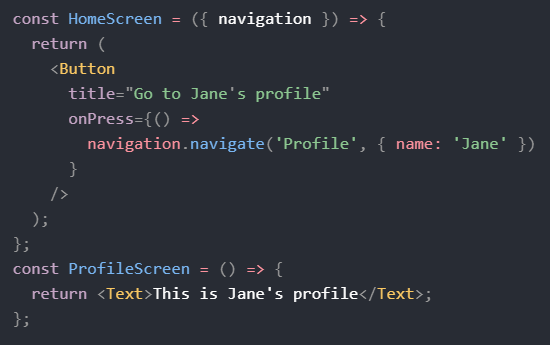
\includegraphics[width=\linewidth]{NavigerenPaginasReactNative.png}
    \caption{Navigeren naar een andere pagina in React Native. Bron:
        reactnative.dev/docs/navigation}
    \label{fig:navigerenReactNative}
\end{figure}

\subsubsection{Flutter}
\label{subsubsec:navigatieFlutter}

Flutter maakt voor de navigatie binnen een applicatie gebruik van de klasse
Navigator. Deze klasse op zich is ook een widget, de bouwstenen van een
applicatie in Flutter. De verschillende pagina's en schermen van een applicatie
worden routes genoemd. Deze routes worden op een stack geplaatst, die de
volgorde van de routes bijhoudt. Er zijn twee verschillende aanpakken van
navigatie binnen Flutter: de ene is gebaseerd op een vaste volgorde waar alle
schermen elkaar opvolgen en de andere laat de ontwikkelaar toe om op aangepaste
wijze te navigeren tussen verschillende pagina's. Beide aanpakken worden in de
volgende paragrafen verder besproken. 

De eerste aanpak laat de gebruiker toe om in een vaste volgorde door de
applicatie te navigeren. Dit is voornamelijk belangrijk als de gebruiker terug
wil gaan naar het vorige scherm. In dit geval is het alleen maar logisch om naar
de vorige route in de stack te gaan. Het is ook meteen de meest eenvoudige vorm
van navigatie. Als de gebruiker naar een andere pagina navigeert wordt deze
bovenaan de stack geplaatst. Indien de gebruiker terug wenst te gaan wordt de
bovenste route terug verwijderd van de stack en komt de gebruiker op de vorige
pagina terecht.

De tweede aanpak is een iets gecompliceerdere aanpak. Deze volgt geen logische
volgorde maar wel de volgorde die vastgelegd is door de ontwikkelaar. De aanpak
berust op een Navigator.pages object. Hieraan kunnen de verschillende pagina's
toegevoegd worden. Vervolgens zal de Navigator dit Navigator.pages object
omzetten in een stack van routes. Indien een nieuwe pagina wordt toegevoegd aan
Navigator.pages dan wordt de stack ook geüpdate. 

\begin{figure}
    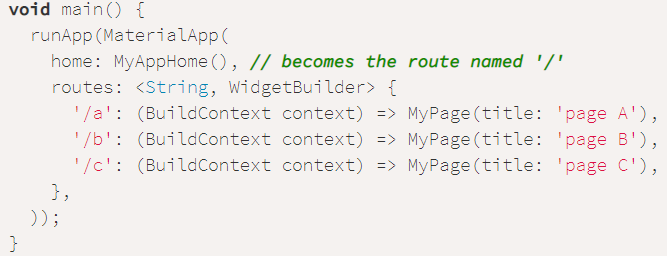
\includegraphics[width=\linewidth]{NamedRoutesFlutter.png}
    \caption{Opzetten navigatie met benoemde routes in Flutter. Bron:
        \textcite{Flutter.dev2020}}
    \label{fig:namedRoutesFlutter}
\end{figure}

\begin{figure}
    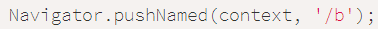
\includegraphics[width=0.5\linewidth]{UseNamedRouteFlutter.png}
    \caption{Benoemde route tonen in Flutter. Bron: \textcite{Flutter.dev2020}}
    \label{fig:useNamedRoutesFlutter}
\end{figure}

Een applicatie kan uit zeer veel verschillende schermen bestaan. Om de navigatie
ertussen overzichtelijk te houden voor de ontwikkelaar beschikt Flutter over een
functie om de routes een naam te geven. Vervolgens kan de pagina aan de hand van
zijn naam getoond worden. In figuur \ref{fig:namedRoutesFlutter} is de definitie
van een map te zien die de naam van een route bevat en de builder die de route
effectief zal tonen op het scherm. In figuur \ref{fig:useNamedRoutesFlutter} is
te zien hoe de route effectief getoond kan worden. Uit de naam van de methode
wordt duidelijk dat ook deze methode gebruik maakt van een stack voor de
navigatie. De nieuwe route wordt bovenop de stack geplaatst.

Beide methodes maken dus gebruik van dezelfde stack en kunnen dus ook door
elkaar gebruikt worden. Dit is een logische aanpak, aangezien een logische
volgorde in een applicatie absoluut noodzakelijk is. Indien een gebruiker terug
wil gaan is het alleen logisch om naar de vorige stap te gaan, ongeacht welke
methode gebruikt werd om naar de huidige pagina te navigeren. 

Verder is het in Flutter mogelijk om een route een waarde te laten terug geven.
Dit is bijvoorbeeld handig indien de gebruiker op oké moet klikken alvorens er
naar het volgende scherm gegaan kan worden. Indien de gebruiker uit dit scherm
gaat door de terug knop van het systeem te gebruiken is de waarde die
teruggegeven wordt null en zal het volgende scherm dus niet getoond worden.

Tot slot geeft de Navigator klasse de ontwikkelaar ook de mogelijkheid om popups
te tonen op het scherm. Dit zijn schermen die niet de volledig oppervlakte van
het scherm in nemen en dus nog een deel van het onderliggende scherm tonen. Het
onderliggende scherm wordt echter geblokkeerd, de gebruiker kan dus enkel binnen
de popup input geven. Deze popups gedragen zich verder als een normale route, de
navigatie naar een popup en er weg van is dus exact hetzelfde.

\subsubsection{Vergelijking navigatie}
\label{subsubsec:vglNavigatie}

Beide frameworks hebben hun eigen techniek om de navigatie aan te pakken. Het
grootste verschil tussen beiden is dat React Native gebruik maakt van een
library, waar Flutter gebruik maakt van een widget. Dit verschil vloeit voort
uit het fundamentele verschil in aanpak tussen beide frameworks. De oorzaak is
dat React Native voor een heel groot deel door de community onderhouden wordt.
Onder andere de library voor navigatie komt voort uit de community en zit dus
niet standaard in React Native, waar dit bij Flutter wel standaard beschikbaar
is.

Voor de volgorde van de navigatie bij te houden maken beide frameworks gebruik
van een stack. Ze zijn dus beide in staat om terug te gaan naar de vorige
pagina. Bij React Native moet elke pagina echter wel steeds benaamd worden om er
naar toe te kunnen navigeren, waar het bij Flutter mogelijk is om op voorhand
een vaste volgorde te definiëren.

In het gevoel voor de gebruiker is er echter geen verschil tussen beide
frameworks. Beide frameworks leveren een navigatie af die overeen komt met de
native navigatie. Verder kan de ontwikkelaar bij beide de overgang tussen de
verschillende pagina's aanpassen om te voldoen aan de uitstraling die de app
wilt geven. 

Er kan besloten worden dat er op het vlak van navigatie geen duidelijk beter
framework is. Er is een verschil tussen de manier waarop de ontwikkelaar de
navigatie implementeerd, maar voor de gebruiker heeft de navigatie met beide
frameworks hetzelfde native gevoel.

\subsection{Toegang native API's}
\label{subsec:toegangNativeAPIs}

Om een applicatie te kunnen afleveren die alle hardware functionaliteiten van
het doelplatform kan gebruiken is het noodzakelijk dat het framework toegang
heeft tot de Native API's van het platform. Ook de manier waarop dit gebeurd is
van belang, hoe efficiënter dit gebeurd, hoe beter de performantie van de
applicatie. Cross-platform frameworks bieden een eigen API aan om met de meest
voorkomende eigenschappen te kunnen werken. Op deze manier hoeven de
ontwikkelaars geen native code of componenten te kennen om een applicatie te
schrijven.

\subsubsection{React Native}
\label{subsubsec:nativeAPIReactNative}

Zoals voor de meeste functionaliteit van het framework rekent React Native op
libraries om specifieke eigenschappen van een platform te kunnen gebruiken. Zo
is er bijvoorbeeld de library React Native Camera. Dit is een library die de
ontwikkelaar toelaat om de camera van een apparaat te gebruiken, ongeacht het
besturingssysteem van het apparaat. Voor de meest voorkomende eigenschappen van
apparaten bestaan er dergelijke libraries. De ontwikkelaar hoeft dus geen native
code te kennen om toch gebruik te kunnen maken van platform specifieke
eigenschappen.

In uitzonderlijke gevallen kan het echter zijn dat de ontwikkelaar een
eigenschap van een bepaald apparaat wil gebruiken waarvoor nog geen library
beschikbaar is. Een applicatie maken die de eigenschappen van een apparaat niet
ten volle gebruikt is uiteraard niet de bedoeling. Om te vermijden dat in dit
geval native ontwikkeling van de applicatie beter zou zijn voorziet React Native
de mogelijkheid om in deze uitzonderlijke gevallen toch native code te gaan
schrijven. Op deze manier kan de ontwikkelaar wel alle eigenschappen gebruiken,
zonder dat het hele project in de native taal geschreven moet worden. De native code wordt omsloten door een native module die ingepast kan worden in de React Native applicatie.

\subsubsection{Flutter}
\label{subsubsec:nativeAPIFlutter}

Flutter maakt voor de toegang tot specifieke eigenschappen van een platform
gebruik van plugins. Zo is er bijvoorbeeld de camera plugin die de ontwikkelaar
toelaat om de camera van een apparaat te gebruiken. De plugin bevat onder meer
methodes om alle beschikbare camera's van een apparaat op te halen (bij een
smartphone bijvoorbeeld de camera aan de voorkant en die aan de achterkant), de
gewenste camera te selecteren en een foto te nemen met deze camera. Voor de
meest voorkomende eigenschappen bestaan er dergelijke plugins. Ook hier hoeft de
ontwikkelaar dus geen native code te kennen om toch specifieke eigenschappen van
een platform te kunnen gebruiken.

Indien de ontwikkelaar eigenschappen van een apparaat wil gebruiken waarvoor nog geen plugin bestaat voorziet Flutter de mogelijkheid om toch native code te gaan schrijven en dit te implementeren in de Flutter applicatie. Flutter voorziet klassen die de communicatie tussen platform-specifieke en Flutter code verzorgen. Deze laten toe om native code te schrijven voor een specifieke toepassing.

\subsubsection{Vergelijking toegang native API's}
\label{subsubsec:vglToegangNativeAPIs}

In de vorige secties werd duidelijk dat beide frameworks de gebruiker in staat stellen om toegang te hebben tot de native API's. Bij beiden zijn er voor de meest voorkomende eigenschappen reeds oplossingen voorzien (bij React Native in de vorm van een library, bij Flutter in de vorm van een plugin). Indien er nog geen standaard oplossing voor bestaat om een bepaalde eigenschap te gebruiken laten beide frameworks de ontwikkelaar toe om alsnog native code te gaan schrijven. De ontwikkelaar heeft dus steeds gegarandeerd toegang tot alle eigenschappen van een apparaat. Kennis van de native code is wel nodig in deze omstandigheden bij beide frameworks.


